

\begin{frame}
    \frametitle{前情回顾}
    \begin{itemize}
        \item 量子化光场~~真空态~~产生湮灭算符 
        \item 相干态~~ 平移算符 ~~相图
        \item 压缩态~~ 压缩算符
        \item 数态表象~~数态展开
        \item 参量下转换~~平衡零差探测 
    \end{itemize}     
\end{frame}

%%%%%%%%%%%%%%%%%%%%%%%%%%%%%%%%%%
\begin{frame} [plain]
    \frametitle{}
    \Background[1] 
    \begin{center}
    {\huge 第10-11讲:光子统计}
    \end{center}  
    \addtocounter{framenumber}{-1}   
\end{frame}
%%%%%%%%%%%%%%%%%%%%%%%%%%%%%%%%%%

\section{1. 光子计数}

\begin{frame}
 \frametitle{计数技术概要}
    {\Bullet} 盖革-米勒计数器
    \begin{center}
        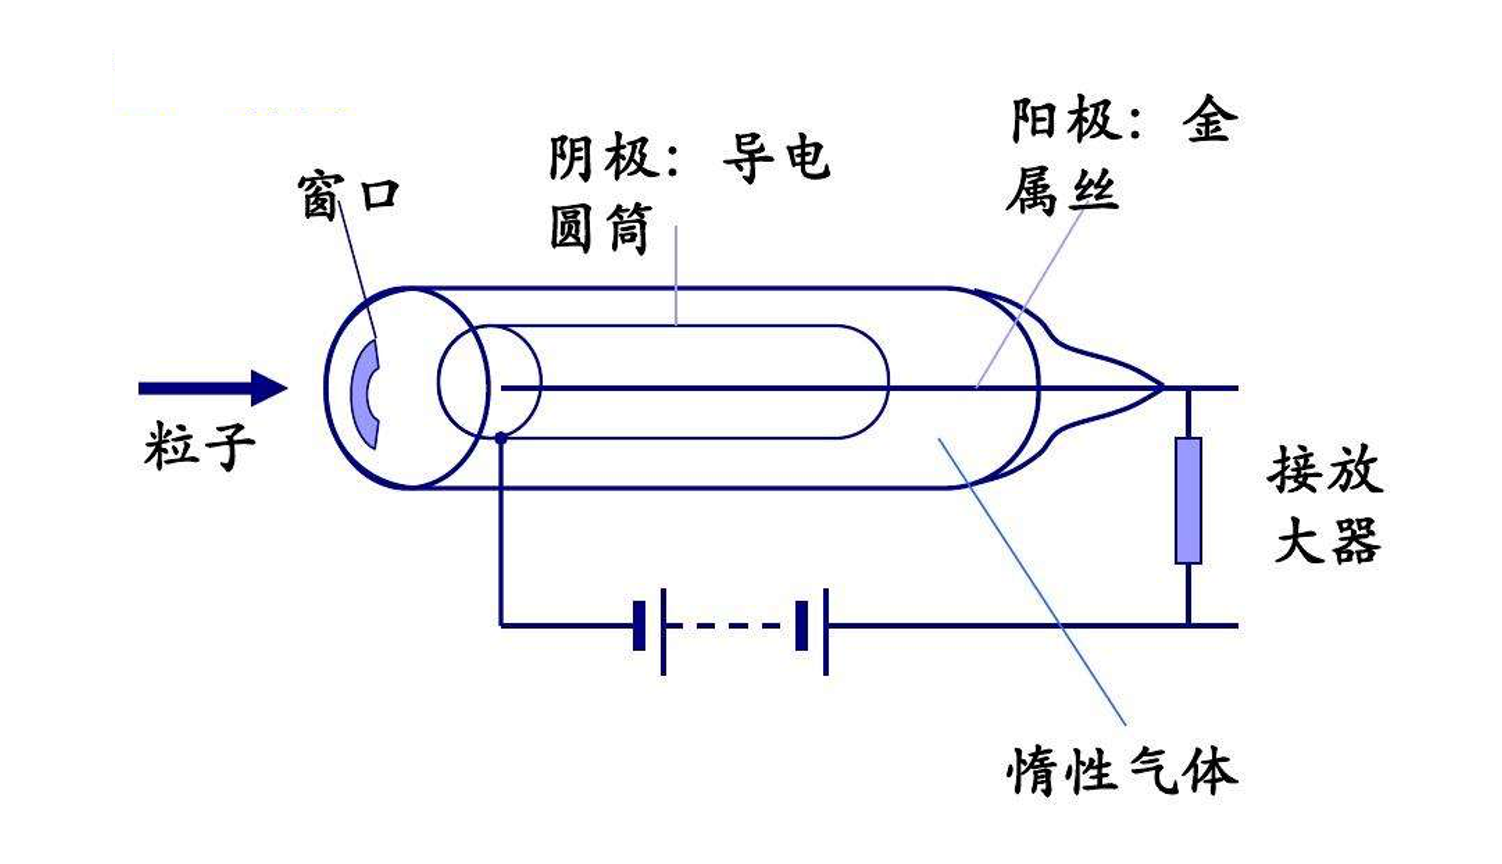
\includegraphics[width=0.7\textwidth]{figs/16.png}
    \end{center}  
\end{frame}

\begin{frame}
 \frametitle{}
 工作原理: 设备初始电压略低于管内稀薄气体击穿电压的, 一个带电粒子射入气体, 原子受激发射紫外光子, 光子射到阴极产生光电子, 光电子向阳极漂移,电离沿途气体,引起离子增殖, 形成自激放电. 输出一个脉冲电流信号.\\  {\vspace*{0.6em}}
      特点: 非常灵敏, 造价低廉、使用方便、探测范围 \\ 
      缺点: 不适合极快速计数, 不能区别粒子类型 \\ 
      著名成果: \\ 
      \begin{enumerate}
          \item 1911年, 卢瑟福用来计数$\alpha$粒子, 提出有核原子模型
          \item 1937年, 测定了宇宙射线的角分布
          \item 目前依然是核物理学和粒子物理学中不可缺少的探测器 
      \end{enumerate}
\end{frame}

\begin{frame}
 \frametitle{}
    {\Bullet} 单光子计数\\  {\vspace*{0.6em}}
    光子流量 ($\varPhi $): 单位时间通过的光子数 \\  光流强度 (P): 单位时间通过的光的能量 \\ 
    对于单色光(频率$\omega $), 有关系式:
    $$ ~~P = \varPhi  \cdot \hbar \omega  $$ \\ 
    当P降低到$10^{-16} W $时, 称为弱光, 可见光子流量约为 ~1~ ms 每光子, 必须考虑单光子计数
\end{frame}

\begin{frame}
      \frametitle{}
      {\Bullet} 真空光电倍增管\\ 
      \begin{center}
           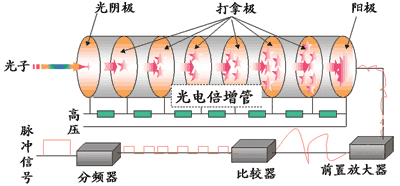
\includegraphics[width=0.6\textwidth]{figs/2022-05-04-16-57-37.png}
      \end{center}
      工作原理: 单光子在光阴极打出一个光电子, 光电子打在第一倍增极并被拿住, 第一倍增极发出数倍的二次电子, ...经数十级打拿增殖, 在阳极回路输出一个脉冲电流信号.  \\ {\vspace*{0.6em}}
    信噪比: (1) 光场的统计涨落, (2) 光阴极热电子, (3) 脉冲堆积效应
\end{frame}

\begin{frame}
 \frametitle{}
    {\Bullet} 雪崩光电二极管\\  {\vspace*{0.6em}}
      \begin{center}
           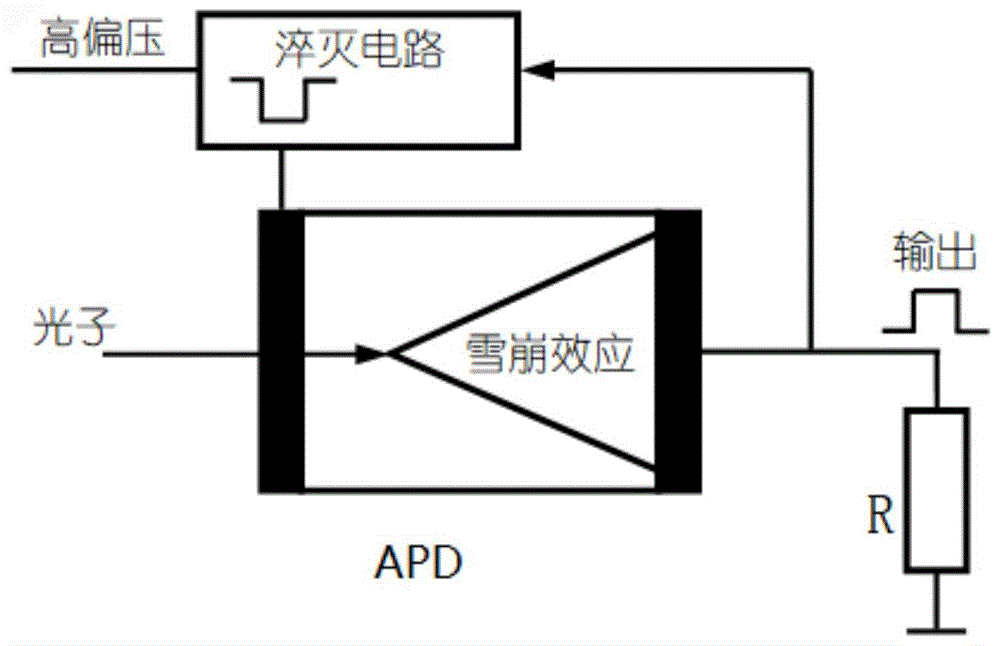
\includegraphics[width=0.45\textwidth]{figs/2022-05-04-18-25-01.png}
      \end{center}

    工作原理: PN 结工作在反向击穿电压附近, 吸收光子时, 光生载流子在强电场下运动,沿途原子电离实现载流子雪崩式增殖, 产生击穿脉冲电流信号.  \\  {\vspace*{0.6em}}

    特点: 在一个探测周期内最多只能完成一次计数. \\ 
    信噪比: (1) 光场的统计涨落, (2) 热生载流子, (3) 脉冲堆积效应 
\end{frame}

\begin{frame}
 \frametitle{}
 {\Bullet} 光场统计分布对计数的影响\\ 
 \begin{enumerate}
     \item 漏掉光子(没有脉冲)
     \item 漏掉计数(没有脉冲峰重叠)
     \item 每次计数窗口的计数不同,波动大.
     \item ...
 \end{enumerate} 
 \begin{center}
      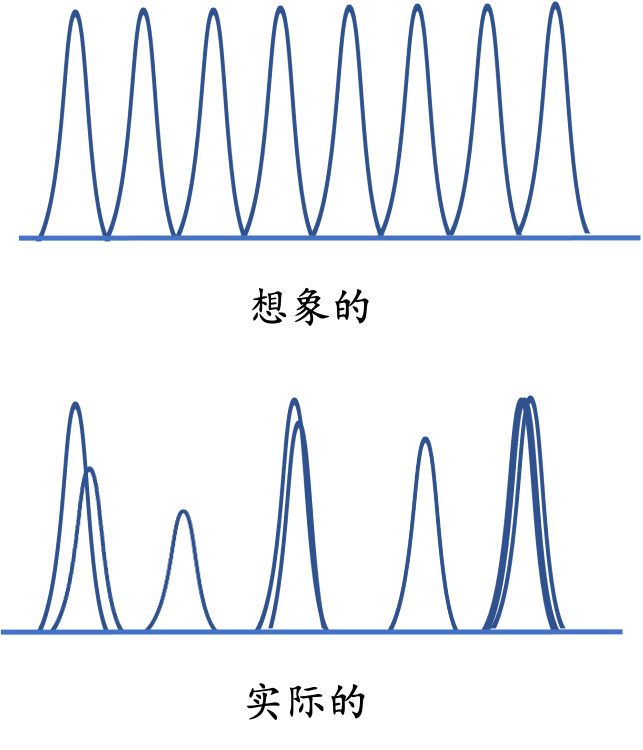
\includegraphics[width=0.35\textwidth]{figs/17.png}
 \end{center} 
\end{frame}

\begin{frame}
 \frametitle{光子计数率}
    光子流量: 
 \[ \varPhi =  \frac{P}{\hbar \omega} = \frac{I A}{\hbar \omega} \, \text{photons} \cdot s^{-1}  \]
    设备的量子效率 ($\eta$), 计数窗口时长为T, 则能被计数的平均光子数: 
    \[\overline{N}(T)=\eta \varPhi T=\frac{\eta P T}{\hbar \omega}\]
    设备的计数率 (count rate): 
    \[ R= \frac{\overline{N}(T)}{T} = \frac{ \eta P }{\hbar \omega} = \eta\varPhi \, \text{counts} \cdot s^{-1} \]
\end{frame}

\begin{frame}
 \frametitle{}
 定性分析: \\ {\vspace*{0.6em}}
      弱光计数:  通常, 量子效率 ($\eta$)约为 10\%, 计数率(R)上限约为 $10^6$ (存在死时间,约为 $1\mu s$), 因此用这种方法能计数的光场强度(P) 上限约为 $10^{-12} W $  \\  {\vspace*{0.6em}}
 定量分析: \\ {\vspace*{0.6em}}
      设一光束的光子能量为 $2.0 eV$, 光流强度为 $1 nW$, 则光子流量: 
      \[ \varPhi =  \frac{P}{\hbar \omega} = \frac{10^{-9}}{2.0 \times 1.6 \times 10^{-19}} = 3.1 \times 10^{9} \, \text{photons} \cdot s^{-1}  \]
      取光速$c=3\times 10 ^8 \, \text{m} \cdot s^{-1} $ , 表明每3米长的光束约中含31个光子. \\ 
      取计数时长 $T= 1 ns$, 对应的光束长度为 $30 cm$, 所含的光子数目约为 $3.1$, 因此光场必须量子化. \\ 
\end{frame}

\begin{frame}
      \frametitle{}
      把光分成多个$30 cm$的光束, 并不是每个光束都含$3.1$个光子, 其统计波动有可能是比较大的, 比如 \\
      \[ 0, 1, 2, 0, 6, 10, 0, 0, \cdots  \]
      如果光束长度为 $3 cm$, 其所含的光子数为$0.31$, 则光子数分布大约长这样:
      \[0,0,1, 1, 0, 0, 0, 1, 2, 0, 0, 0, \cdots \]
      此时, {\color{red}{光子的统计分布}}对计数的影响是决定性的
\end{frame}

\section{ 2. 三类统计光场}

\begin{frame}
 \frametitle{推导}
      考虑经典单色光场: 
      \[ E(x,t) = E_0 \sin (k x - \omega t + \varphi )\]
      一个理想的单模激光器发出的正是这种光, 称为相干光. 它的能量(光强)为:
      \[ <I> = \frac{1}{2} c \epsilon_0 n E_0 ^2\]
      考虑一个长为 L 光束, 其光流强度P是常数, 则所含的平均光子数为:
      \[\overline{n} = \varPhi \cdot \frac{L}{c} \]
      现在把它分成N段, 每段长度为 $L/N$, 当 $N\gg \overline{n} $时, 在不计一段有多个光子的低概率事件条件下,则在某段找到一个光子的概率为 
      \[ p= \frac{\overline{n}}{N} \] 
      现在的情况就是有 $n$ 个段含(一个)光子, (N-n)段不含光子. 
\end{frame}

\begin{frame}
      \frametitle{}
      ~\\
      这是一个N个独立的成功(含光子)/失败(不含光子)试验模型, 每次试验成功的概率为$p$, 则成功次数($n$)的离散概率分布服从二项分布
      \[ P(n) = C^n _N  p^n (1-p)^{N-n} \]
    \begin{center}
             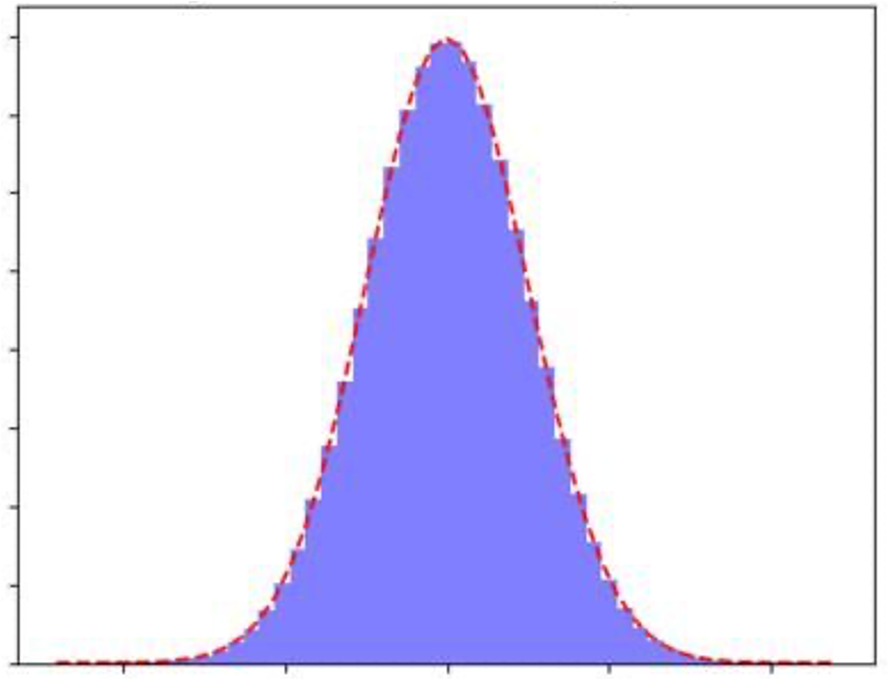
\includegraphics[width=0.5\textwidth]{figs/18.png}
    \end{center}
\end{frame}

\begin{frame}
      \frametitle{}
    把 $p= \dfrac{\overline{n}}{N}$ 代入, 有
      \[\begin{aligned}
          P(n) &= C^n _N  p^n (1-p)^{N-n} \\ 
             &= \frac{N!}{n! (N-n)!} p^n (1-p)^{N-n} \\ 
             &=  \frac{N!}{n! (N-n)!} (\frac{\overline{n}}{N} ) ^n (1-\frac{\overline{n}}{N})^{N-n} \\ 
             &= \frac{1}{n!} \left(\frac{N!} {(N-n)!N^n} \right) \overline{n}^n (1-\frac{\overline{n}}{N})^{N-n}  , 
      \end{aligned}\]
      取 $ N \to \infty , \cdots $
    \end{frame}

\begin{frame}
 \frametitle{}
    利用斯特林公式 
       \[\lim _{N \rightarrow \infty}[\ln N !]=N \ln N -N \]
    有: 
       \[\begin{aligned}
        \lim _{N \rightarrow \infty}\left[ \ln \left(  \frac{N!} {(N-n)!N^n} \right) \right]  &=  0 \\ 
        \lim _{N \rightarrow \infty}\left(  \frac{N!} {(N-n)!N^n} \right) &= 1  \qquad  \cdots (1)
    \end{aligned}\]
    利用公式 
    \[\lim _{N \rightarrow \infty} \left( 1-\frac{1}{N} \right)^N =\frac{1}{e}\]
    \[\begin{aligned}
        \lim _{N \rightarrow \infty} \left(1-\frac{\overline{n}}{N} \right)^{N-n}&=   \lim _{N \rightarrow \infty} \left(1-\frac{1}{N / \overline{n}} \right)^{(N / \overline{n}) \overline{n}}\\ 
         & = e^{-\overline{n}} \qquad  \cdots (2)
    \end{aligned}\]
\end{frame}

\begin{frame}
 \frametitle{}
      把(1)(2)代回, 有: 
      \[\begin{aligned}
        P(n) &= \frac{1}{n!} \overline{n}^n e^{-\overline{n}}  \\ 
        &= \frac{\overline{n}^n}{n!} e^{-\overline{n}}, \qquad (n=0, 1, 2, \cdots )
    \end{aligned}\]
    正是相干光场Fock态表中推导的泊松公布!, 且有:
    \[ \overline{n}= \left|\alpha\right|^2\]
    说明: 相干态光场是真随机等概率分布光场
\end{frame}

\begin{frame}
 \frametitle{定性分析}
     (1)  泊松公布要求试验次数(n) 为非负整数. \\ 
     {\Bullet}光子数只能是非负整数 \\ {\vspace*{0.3em}}
     (2)  泊松公布要求每次试验成功的概率相同. \\ 
     {\Bullet}随着N的增加, 光束在能量空间被分成一个个的波包, 相干态光子真随机等概率分布. \\ {\vspace*{0.3em}}
     (3)  取 $ N \to \infty $ 相当于经典长度无限可分. 有量子长度最小, 到达最小长度,即取得最大的N
     (4)  泊松公布要求每次试验是相互独立的. 即前一次试验结果不影响后面的试验. \\ 
     {\Bullet}光子是玻色子, 前一个光子的占据情况不影响后一个光子. \\ {\vspace*{0.3em}}
\end{frame}

\begin{frame}
 \frametitle{定量分析}
    * 分布的归一性: 
    \[\begin{aligned}
        P(n) &= \frac{\overline{n}^n}{n!} e^{-\overline{n}} \\ 
        \sum_{n=0} ^{\infty} P(n) &= \sum_{n=0} ^{\infty}\frac{\overline{n}^n}{n!} e^{-\overline{n}}  \\ 
        &= e^{-\overline{n}} \sum_{n=0} ^{\infty}\frac{\overline{n}^n}{n!} \\ 
        &= e^{-\overline{n}} \left( 1+ \overline{n} + \frac{\overline{n}^2}{2!} +\frac{\overline{n}^3}{3!} + \cdots \right) \\ 
        &= e^{-\overline{n}} \times e^{\overline{n}}  \\ 
        &= 1
    \end{aligned}\]   
\end{frame}

\begin{frame}
 \frametitle{}
  (1) 密度矩阵: 
  \[\begin{aligned} 
 \rho &=\rl{\alpha}{\alpha} \\ 
 &= \sum P(n) \rl{n}{n} \\ 
 & = \sum \frac{\overline{n}^n}{n!} e^{-\overline{n}} \rl{n}{n}  \\ 
 & = \sum \frac{\left|\alpha\right|^{1n}}{n!} e^{-\left|\alpha\right|^2} \rl{n}{n}  \\ 
\end{aligned}\] 
\end{frame}

\begin{frame}
 \frametitle{}
 (2) 均值:
 \[\begin{aligned} 
    \overline{n}  \equiv  Tr(\rho a^{\dagger} a) & \equiv  \sum_{n=0} ^{\infty} n  P(n) \\ 
    &= e^{-\overline{n}} \sum_{n=0} ^{\infty} n \frac{\overline{n}^n}{n!} \\ 
    &= e^{-\overline{n}} \left( 0+ \overline{n} + 2\frac{\overline{n}^2}{2!} +3\frac{\overline{n}^3}{3!} + \cdots \right) \\  
    &= \overline{n} e^{-\overline{n}} \left( 1+ \overline{n} + 2\frac{\overline{n}^2}{2!} +3\frac{\overline{n}^3}{3!} + \cdots \right) \\ 
    &= \overline{n} e^{-\overline{n}} \times e^{\overline{n}}  \\ 
    &= \overline{n} 
\end{aligned}\]     
\end{frame}

\begin{frame}
 \frametitle{}
   (3) 递推式: 
 \[\begin{aligned}
     P(n) &= \frac{\overline{n}^n}{n!} e^{-\overline{n}} \\ 
     &= \frac{\overline{n}^{n-1} \overline{n} }{(n-1)! n} e^{-\overline{n}} \\ 
     &= \frac{\overline{n}}{n}\frac{\overline{n}^{n-1}  }{(n-1)! } e^{-\overline{n}} \\ 
     &= \frac{\overline{n}}{n} P(n-1)\\ 
 \end{aligned}\]   
  表明:
  \begin{enumerate}
      \item $P(n)> P(n-1), \text{if} \quad  \overline{n}> n $
      \item $P(n)< P(n-1), \text{if} \quad \overline{n}< n $
  \end{enumerate}
\end{frame}

\begin{frame}
 \frametitle{}
     (4) 方差(variance): (涨落)
      \[\begin{aligned}
        Var(n) &= \overline{ (\Delta n)^2 }  \\ 
        &= \overline{ n^2} - \overline{n}^2 \\
        &= \sum_{n=0} ^{\infty} n^2 P(n) -\overline{n}^2 \\ 
        &= \sum_{n=0} ^{\infty} (n^2-n) +n P(n) -\overline{n}^2 \\ 
        &= \sum_{n=0} ^{\infty} n(n-1) P(n) + \overline{n} -\overline{n}^2 \\
    \end{aligned}\]  
\end{frame}

\begin{frame}
 \frametitle{}
 \[\begin{aligned}
    \sum_{n=0} ^{\infty} n(n-1) P(n)  & =  \sum_{n=0} ^{\infty} n(n-1) \frac{\overline{n}^n}{n!} e^{-\overline{n}}  \\
    &= e^{-\overline{n}} \sum_{n=0} ^{\infty} n(n-1) \frac{\overline{n}^n}{n!} \\ 
    &= e^{-\overline{n}} (0+0+ 2 \frac{\overline{n}^2}{2!} +  6 \frac{\overline{n}^3}{3!} + \cdots  ) \\ 
    &= \overline{n}^2 e^{-\overline{n}} (1 +  6 \frac{\overline{n}^1}{3!} + 12 \frac{\overline{n}^2}{4!}  \cdots  ) \\ 
    &= \overline{n}^2 e^{-\overline{n}} (1+ \overline{n} +  2 \frac{\overline{n}^2}{2!} + 3 \frac{\overline{n}^3}{3!}  \cdots  ) \\ 
    &= \overline{n}^2 e^{-\overline{n}} \sum_{n=0} ^{\infty} \frac{\overline{n}^n}{n!} = \overline{n}^2 \sum_{n=0} ^{\infty}  P(n)\\ 
    & = \overline{n}^2
\end{aligned}\]  
\end{frame}

\begin{frame}
    \frametitle{}
         \[\begin{aligned}
            \overline{ (\Delta n)^2 }  &= \sum_{n=0} ^{\infty} n(n-1) P(n) + \overline{n} -\overline{n}^2 \\
           &= \overline{n}^2  + \overline{n} -\overline{n}^2 \\ 
           &= \overline{n}
       \end{aligned}\]  
   \end{frame}

   \begin{frame}
    \frametitle{}
     (5) 标准偏(standard deviation)
     \[ \Delta n = \sqrt{\overline{ (\Delta n)^2 }}  = \sqrt{\overline{n}}  =\left|\alpha\right|  \]
     波动(fluctuations):
     \[ \frac{\Delta n}{n}\]
     随着光子平均数的增大, 统计波动变得越来越小
\end{frame}

\begin{frame}
      \frametitle{特点: 平均粒子数唯一决定泊松光场的数态分布}
      \[P(n) = \frac{\overline{n}^n}{n!} e^{-\overline{n}}, \qquad \overline{ (\Delta n)^2 } = \overline{n}, \qquad  \Delta n = \sqrt{\overline{n}}, \qquad \overline{n}= \left|\alpha\right|^2\]
       \begin{center}
            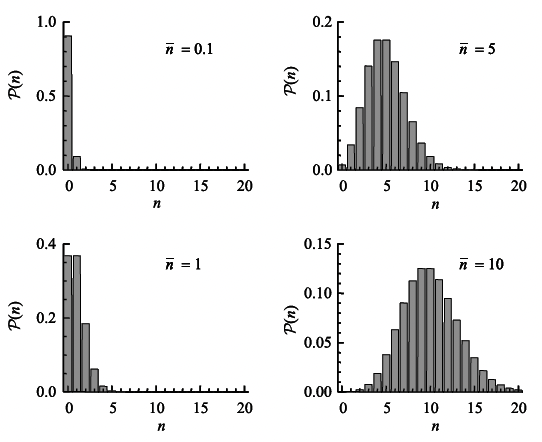
\includegraphics[width=0.53\textwidth]{figs/2022-05-06-09-01-55.png}
       \end{center}
   \end{frame}

%%%%%%%%%%%%%%%%%%%%%%%%%%%%%%%%%%%%%%%%%%%%%%%%%%%%%%%%%%%%%%%%%%%
\begin{frame}
    \frametitle{课堂作业}
     \begin{block}{ 1. An attenuated beam from an argon laser operating at
        514 nm (2.41 eV) with a power of 0.1 pW is detected with a photoncounting
        system of quantum efficiency 20\% with the time interval set at
        0.1 s. \\
        {\hspace*{1.5em}} Calculate (a) the mean count value, and (b) the standard deviation
        in the count number.}
     \end{block}
\end{frame}
%%%%%%%%%%%%%%%%%%%%%%%%%%%%%%%%%%%%%%%%%%%%%%%%%%%%%%%%%%%%%%%%%%%
 
\begin{frame}
 \frametitle{}
      \解~激光是相干光,服从泊松分布\\ 
      光子流量: 
      \[ \varPhi =  \frac{P}{\hbar \omega} = \frac{10^{-13}}{2.41 \times 1.6 \times 10^{-19}} = 2.59 \times 10^{5} \, \text{photons} \cdot s^{-1}  \]
      平均粒子数: 
      \[\overline{n}(T)=\eta \varPhi T= 0.2 \times 2.59 \times 10^{5} \times 0.1 =  5180 \]
      标准偏: 
      \[ \Delta n = \sqrt{\overline{n}} = 72   \]
\end{frame}

\begin{frame}
 \frametitle{三种统计}
      一个完美的相干光场,光子数服从泊松分布规律. 特点:  \[ \Delta n = \sqrt{\overline{n}}    \]
      因此, 基于标准偏与平均光子数的关系, 光场统计分为三类:
      \begin{enumerate}
          \item 亚泊松统计 (sub-Poissonian statistics) 
          \[ \Delta n < \sqrt{\overline{n}}    \]
          \item 泊松统计 (Poissonian statistics)
          \[ \Delta n = \sqrt{\overline{n}}    \]
          \item 超泊松统计 (super-Poissonian statistics)
          \[ \Delta n > \sqrt{\overline{n}}    \]
      \end{enumerate}
\end{frame}

\begin{frame}
 \frametitle{}
 \begin{center}
    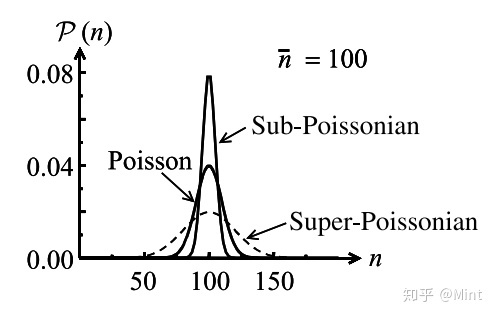
\includegraphics[width=0.6\textwidth]{figs/2022-05-06-10-46-42.png}
\end{center}
方差: 越小, 分布越集中, 说明系统越稳定. 因此, 稳定性关系为: \\ 
\[\text{亚泊松统计} > \text{泊松统计} > \text{超泊松统计} \]
\end{frame}

\begin{frame}
 \frametitle{三种光场}
 \begin{enumerate}
    \item 亚泊松光场: 非经典光场 (单光子源, 压缩态,光子反聚束, Fock态光 ,$\cdots$)
    \[ 0 \leq \Delta n < \sqrt{\overline{n}}    \]
    \item 泊松光场: 相干光场面(理想激光器)  
    \[ \Delta n = \sqrt{\overline{n}}    \]
    \item 超泊松光场: 经典光场(非理想激光器, 混沌光束, 光子聚束, 热辐射场,$\cdots$ )
    \[ \Delta n > \sqrt{\overline{n}}    \]
\end{enumerate}
    * 相干光做为泊松光是最接近经典光的量子光, 也是最接近量子光的经典光! \\ 
    * 非经典光压缩了相干光的展宽(压缩态); 相干光的展宽对应着恒定光强~ $I(t)=I(0)$ ; 经典光阔展了相干光的展宽,对应非恒定光流强度~ $I(t) \not = I(0)$, 即存在光子数波动 . 
\end{frame}

\begin{frame}
 \frametitle{~1. 单模热光场}
    热体辐射的电磁场称为热光场, 也称黑体辐射场. \\ 
    黑体可看成一系列的谐振子. 考虑一个频率为$\omega$的谐振子激发的单模光场, 能量为:
    \[ E_n = (n+\frac{1}{2}) \hbar \omega \] 
    考虑光子数服从玻尔兹曼分布
    \begin{equation*}
        P(n) =\frac{N_{n}}{N}=\frac{\exp \left(-\frac{E_{n}}{k_B T}\right)}{\sum_{n} \exp \left(-\frac{E_{n}}{k_B T}\right)}
    \end{equation*}
\end{frame}

\begin{frame}
 \frametitle{}
 代入能量(不考虑真空能):
    \[\begin{aligned}
     P(n) &=\frac{\exp \left(-\frac{n \hbar \omega }{k_B T}\right)}{\sum_{n} \exp \left(-\frac{n \hbar \omega }{k_B T}\right)} \\ 
     &= \frac{\exp^n \left(-\frac{\hbar \omega }{k_B T}\right)}{\sum_{n} \exp^n \left(-\frac{\hbar \omega }{k_B T}\right)} \\ 
     &= \frac{x^n}{\sum_{n} ^\infty x^n } \\ 
     x&= \exp \left(-\frac{\hbar \omega }{k_B T}\right) <1
    \end{aligned} \]
运用等比列数列求各公式
\[ S_n= \frac{a_1(1-q^n)}{1-q} \]
    \[\sum_{n} ^\infty x^n = \frac{x^0(1-x^n)}{1-x} = \frac{1}{1-x}\] 
\end{frame}

\begin{frame}
 \frametitle{}
 \[\begin{aligned}
    P(n) &= \frac{x^n}{\sum_{n} ^\infty x^n } \\ 
    &= x^n (1-x) \\ 
   \end{aligned} \]
   \[\begin{aligned}
    \overline{n} &= \sum_{n} ^\infty  n P(n)  \\ 
    &= \sum_{n} ^\infty  n x^n (1-x) \\ 
    &= (1-x)x \frac{\mathrm{d} }{\mathrm{dx}}\left( \sum_{n} ^\infty x^n \right)  \\
    &=  (1-x)x \frac{\mathrm{d} }{\mathrm{dx}}\left( \frac{1}{1-x} \right) \\
    &=  (1-x)x \frac{1} {1-x^2} = \frac{x}{1-x} \\ 
   \end{aligned} \]
\end{frame}

\begin{frame}
    \frametitle{}
    \[\begin{aligned}
        x & = \frac{\overline{n}}{\overline{n}+1} \\ 
        &~\\
        P(n) &= x^n (1-x) \\ 
        &=  \frac{1}{\overline{n}+1}\left( \frac{\overline{n}}{\overline{n}+1} \right)^n \\ 
        &=  \frac{\overline{n}^n}{(1+\overline{n})^{n+1}} \\ 
        &= \left( 1-\exp(-\frac{\hbar \omega}{k_B T} )
  \right) \exp(-n \frac{\hbar \omega}{k_B T}) 
      \end{aligned} \]
    称为玻色-爱因斯坦分布. \\  {\vspace*{2.3em}}
\end{frame}

\begin{frame}
 \frametitle{特点分析}
  (1) 分布
  \[ P(n) =\frac{1}{\overline{n}+1}\left( \frac{\overline{n}}{\overline{n}+1} \right)^n \]  
  最大值总出现在$n=0$处,  随着n的增加, 呈指数衰减.
    \begin{center}
         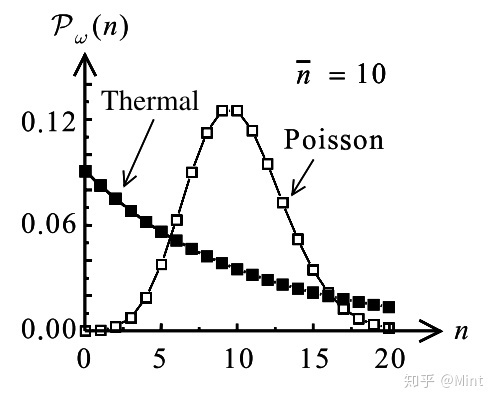
\includegraphics[width=0.4\textwidth]{figs/2022-05-06-14-46-00.png}
    \end{center}    
\end{frame}

\begin{frame}
    \frametitle{}   
    (2) 密度算符 
    \[ \begin{aligned}
        \rho &= \sum _n P(n) |n\left\rangle \right\langle n| \\
        &= \left( 1-\exp(-\frac{\hbar \omega}{k_B T} )
        \right) \sum _n \exp(-n \frac{\hbar \omega}{k_B T}) |n\left\rangle \right\langle n| \\ 
        &= \left( 1-\exp(-\frac{\hbar \omega}{k_B T} )
        \right) \exp(- \frac{\hbar \omega}{k_B T} a^{\dagger} a) \\
        &= \sum_n \frac{(\overline{n})^n}{(1+\overline{n})^{n+1}} |n\left\rangle \right\langle n| \\
        &= \frac{(\overline{n})^{a^{\dagger} a}}{(1+\overline{n})^{a^{\dagger} a+1}} 
    \end{aligned}\] 
\end{frame}

\begin{frame} 
\frametitle{}
    (3) 均值: (正是统计物理学的玻色分布, 化学势 $\mu=0 $)
    \[ \overline{n} \equiv Tr(\rho a^{\dagger} a) = \frac{x}{1-x} = \frac{1}{\exp(\hbar \omega / k_B T) -1}  \] 
     * 均值与温度存在直接的函数关系! \\ 
     ~\\ 
    (4) 方差(涨落):
    \[ Var(n) \equiv \overline{ (\Delta n)^2 } \equiv \overline{ n^2 } - \overline{ n }^2  = \overline{ n }^2 + \overline{ n }\]   
    表明热光场的量子涨落比相干光大出一个$\overline{ n }$ 
   \end{frame}

   \begin{frame}
    \frametitle{}
        计算细节:
    \[\begin{aligned}
        \overline{n^2} &= \sum_{n} ^\infty  n^2 P(n)  \\ 
        &= \sum_{n} ^\infty  n^2 P(n) \\ 
        &= \sum_{n} ^\infty  (n^2-n +n) P(n) \\ 
        &= \sum_{n} ^\infty  (n-1)n  P(n)  + \sum_{n} ^\infty  n  P(n)  \\    
        &= \overline{(n-1)n}  + \overline{n}   
    \end{aligned} \]     
   \end{frame}

   \begin{frame}
    \frametitle{}
    \[\begin{aligned}
        \overline{(n-1)n } &= \sum_{n} ^\infty  (n-1)n  P(n)   \\ 
        &= \sum_{n} ^\infty  (n-1)n  x^n (1-x)  \\    
        &= (1-x)x^2 \frac{\mathrm{d}^2 }{\mathrm{dx^2}}\left( \sum_{n} ^\infty x^n \right)  \\
        &=  (1-x)x \frac{\mathrm{d}^2 }{\mathrm{dx^2}}\left( \frac{1}{1-x} \right) \\
        &=  2 \overline{n}^2\\ 
    \end{aligned} \]   
     \[ Var(n) \equiv \overline{ n^2 } - \overline{ n }^2  = \overline{(n-1)n}  + \overline{n} - \overline{ n }^2= \overline{ n }^2 + \overline{ n }\]  
   \end{frame}

   \begin{frame} 
    \frametitle{}
    黑体辐射场的能量密度由普朗克公式给出:
    \[\begin{aligned}
        \rho(\omega, T) d \omega &=\frac{\hbar \omega ^3}{\pi ^2 c^{3}} \frac{1}{e^{\hbar \omega / K_B T}-1} d \omega \\ 
        &= \frac{\hbar \omega ^3}{\pi ^2 c^{3}} d \omega \overline{n}  \\
        &= \frac{ \omega ^2}{\pi ^2 c^{3}} \overline{\varepsilon}(\omega) d \omega \\ 
        &= g(\omega)d \omega \overline{\varepsilon}(\omega)  
    \end{aligned}\]
    普朗克公式给出的正是光子数分布和光子数密度
   \end{frame}

   \begin{frame} 
    \frametitle{}
     根据统计物理力学, 热涨落源于能量对时间的微分
    \[\begin{aligned}
        \overline{ (\Delta E)^2 }  &= k_B T^2 \frac{\partial \overline{E} }{\partial T } \\ 
        \overline{ (\Delta E)^2 } d \omega &= k_B T^2 \frac{\partial  }{\partial T } (V \rho(\omega, T)  d \omega)  \\
   &= k_B T^2 V d \omega \frac{\partial \rho(\omega, T) }{\partial T } \\ 
   &= (\hbar \omega \rho  + \frac{\pi ^2 c^{3}}{\omega ^2} \rho^2) V d \omega
    \end{aligned} \]    
   \end{frame}

   \begin{frame} 
    \frametitle{}
    热涨落也源于粒子数的涨落
    \[\begin{aligned}
        \overline{ (\Delta E)^2 } d \omega &= g(\omega)d \omega \times \overline{ (\Delta \varepsilon)^2 } \times V \\ 
        &= \frac{ \omega ^2}{\pi ^2 c^{3}} d \omega \overline{ (\Delta (n\hbar \omega))^2 } \times V \\ 
        &= \frac{ \omega ^2}{\pi ^2 c^{3}} \overline{ \Delta (n)^2 } (\hbar \omega)^2 V d \omega 
    \end{aligned} \]  
    两式比较, 得:
    \[\begin{aligned}
        \overline{ \Delta (n)^2 } &=  \frac{\pi ^2 c^{3}}{\hbar \omega ^3}\rho + (\frac{\pi ^2 c^{3}}{\hbar \omega ^3}\rho )^2 \\ 
        &=  \frac{\pi ^2 c^{3}}{\hbar \omega ^3} \frac{\hbar \omega ^3}{\pi ^2 c^{3}} \overline{n}  + (\frac{\pi ^2 c^{3}}{\hbar \omega ^3}\frac{\hbar \omega ^3}{\pi ^2 c^{3}} \overline{n}  )^2 \\ 
        &= \overline{n} + \overline{n}^2
    \end{aligned} \]
    体现了涨落的波粒二象性本质: 粒子性项 $\overline{ n }$,  波动性项 $\overline{ n }^2$ 
   \end{frame}

   \begin{frame} 
    \frametitle{}
    * 若 n 是连续变量, 则应只体现波动性. 
    \[  P(n) =\frac{N_{n}}{N}=\frac{\exp \left(-\frac{n\hbar \omega }{k_B T}\right)}{ \int_{n=0} ^\infty dn \exp \left(-\frac{n\hbar \omega}{k_B T}\right)} = \frac{e^{-nx}}{\int_{n=0} ^\infty  e^{-nx} dn}\]
    \[ \overline{n } = \int_{n=0} ^\infty n P(n)  dn = \int_{n=0} ^\infty n \frac{e^{-nx}}{\int_{n=0} ^\infty  e^{-nx}dn}  dn\]
    \[ \overline{n^2 } = \int_{n=0} ^\infty n^2 \frac{e^{-nx}}{\int_{n=0} ^\infty  e^{-nx}dn}  dn = 2 \overline{n }^2 \]
    \[ Var(n) \equiv \overline{ n^2 } - \overline{ n }^2  = 2\overline{ n }^2 - \overline{ n }^2 = \overline{ n }^2 \] 
    只有波动性带来的项 $\overline{ n }^2$ , 没有了粒子性带来的项 $\overline{ n }$  
\end{frame}

\begin{frame} 
    \frametitle{~2.多模热光场}
    单模热光场是一阶相干的, (任何单模激发的光场都是一阶相干的) . \\
    实际上, 热激发的是多模场, 设模式数目为$n_k$, 则密度算符 
    \[ \begin{aligned}
        \rho &= \sum_{\{n_k\}} |\{n_k\} \left\rangle \right\langle \{n_k\} | \prod_k
        \frac{(\overline{n_k})^{n_k}}{(1+\overline{n_k})^{n_k+1}} \\
    \end{aligned}\] 
    由于各模相位不同, 削弱了波动性带来的涨落:
    \[ \overline{ (\Delta n)^2 } = \frac{\overline{ n }^2}{n_k} + \overline{ n } \] 
    当  $n_k \to \infty$, 热光场趋于泊松分布. \[ \overline{ (\Delta n)^2 } = \overline{ n }\] 
\end{frame}

\begin{frame} 
 \frametitle{~3. 混沌光束}
 实验室常用的两种光源:
 \begin{enumerate}
     \item 激光器: 相干泊松光
     \item 气体放电管: 部分相干混沌光
 \end{enumerate}
   \begin{center}
        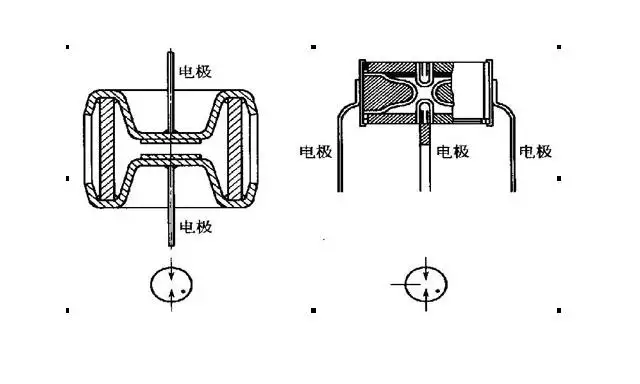
\includegraphics[width=0.7\textwidth]{figs/2022-05-07-11-10-12.png}
   \end{center}
\end{frame}

\begin{frame}
 \frametitle{}
 混沌光束是部分相干光, 光子流量不是常数($\varPhi (t) $) 
 探测器的计数率 (计数期内探测到的光子数):  
    \[R(t)= \int _{t=0} ^ {T} \eta \varPhi (t)  dt\]
 有均值:
\[ \overline{n}  = < R(t)> \]
\[ \overline{n^2}  = < R^2 (t)> \]
均方差:
\[\begin{aligned}
    \overline{(\Delta n)^2} &= < R^2 (t)> - < R(t)>^2 \\ 
    &= \overline{R}(t)+\overline{R}^2(t)
\end{aligned}\]
\end{frame}

\begin{frame}  
 \frametitle{分析}
 \begin{itemize}
     \Item 如果测量时间(T)与相干时间$\tau_c$ 相当, 第二项的影响会很大. 服从超泊松统计.
     \Item 如果$T\gg \tau_c$, 第二项因相位平均趋零,即波动性影响消失. 服从泊松统计.
 \end{itemize}    
\end{frame}

\begin{frame} 
 \frametitle{4. Fock态光场}
 对于相干光,光子流量是常数. 当测量时间(T)变得足够短, 短到每次测得的光子数刚好为1. 
   \begin{center}
        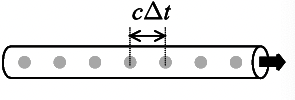
\includegraphics[width=0.4\textwidth]{figs/2022-05-07-14-58-04.png}
   \end{center}
 则相当于单光子源. 变成Fock态光场 \\
 有均值(数密度):
 \[ \overline{n}= Tr(\rho a^{\dagger} a)= n\] 
 方差 (涨落): 
 \[ Var(n) = \overline{(\Delta n)^2} =0 \]
\end{frame}

\begin{frame} 
 \frametitle{损耗导致光场统计退化}
    光束通过光学损耗材料会损失光子, 可以用光学分束器来模拟
      \begin{center}
           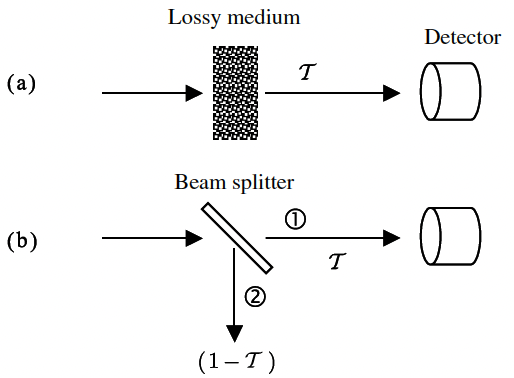
\includegraphics[width=0.6\textwidth]{figs/2022-05-07-15-10-50.png}
      \end{center}      
\end{frame}

\begin{frame} 
 \frametitle{}
    光学分束器模型有可有效表述如下现象:
 \begin{itemize}
    \Item 光源发出的光子没有被全部收集.
    \Item 光的吸收, 光的反射, 光的散射等导致的光子损失.
    \Item 光学探测器的量子效应低导致某些光子没有被探测到.
\end{itemize} 
\end{frame}

\begin{frame} 
 \frametitle{}
   \begin{center}
        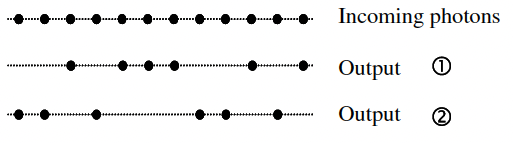
\includegraphics[width=0.7\textwidth]{figs/2022-05-07-15-17-44.png}
   \end{center}
\begin{itemize}
    \item 入射光束的光子流量是常数(相干光), 光子被光随机损耗后, 出射光束的光子流量不再是常数. 
    \item 对于透射率很小的材料, 出射光束的光子流量完全变成了关于时间的随机函数, 变成了非相干光(退相干).
\end{itemize} 
* 光场的统计特性决定于两方面: (1)  光束本身的统计特性, (2) 探测器   
\end{frame}

\section{ 3. 光的探测理论}

\begin{frame} 
 \frametitle{半经典探测理论}
 半经典理论认为: 光束是一系列电磁波构成, 也是一束光子流. 电磁波强度对应光子数
   \begin{center}
        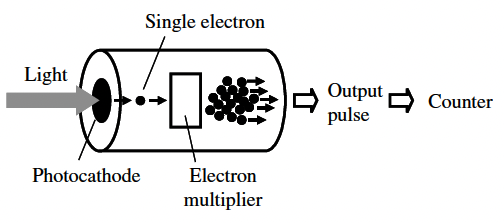
\includegraphics[width=0.7\textwidth]{figs/2022-05-07-15-48-38.png}
   \end{center}      
\end{frame}

\begin{frame} 
 \frametitle{}
    设电磁波强度为$I(t)$, 在  $ \Delta t $ 时间内,测到一次光电发射事件的概率为 
    \[ P (1:, t, t+\Delta t) = \xi I(t) \Delta t \]
    只要$ \Delta t \to 0$, 同时测得两次或两次以上的光电发射事件的概率几乎为零. 因此, 没有测到光电发射事件的概率为 
    \[ P (0:, t, t+\Delta t) = 1- P (1:, t, t+\Delta t) =1- \xi I(t) \Delta t \]
    在$0, t+ \Delta t$时间段内, 测得$n$次光电发射事件的概率为:
    \[\begin{aligned}
        P (n:, 0, t+\Delta t) &= P (n:, 0, t) P (0:, t, t+\Delta t) + P (n-1:, 0, t) P (1:, t, t+\Delta t) \\ 
        &= P (n:, 0, t) (1- \xi I(t) \Delta t ) + P (n-1:, 0, t) \xi I(t) \Delta t 
    \end{aligned}\]
    
\end{frame}

\begin{frame} 
 \frametitle{}
 令 \[ P_n (t)= P (n:, 0, t), \qquad P_n (t+\Delta t)=P (n:, 0, t+\Delta t)\]
 上式可改定为:
 \[ \frac{P_n (t+\Delta t)- P_n (t)}{\Delta t } =\xi I(t) [P_{n-1} (t) -P_{n} (t) ]  \]  
 令$ \Delta t \to 0$, 得微分形式:
 \[ \frac{\mathrm{d}P_n (t)}{\mathrm{d}t} =\xi I(t) [P_{n-1} (t) -P_{n} (t) ]  \]
 令$P_0 (0)=0$, 解方程得:
\[ P_n (t) = \frac{\left[ \int_0 ^t \xi I(t') d t' \right]^n }{n!} \mathrm{e}^{- \int_0 ^t \xi I(t') d t'  } \]
\end{frame}

\begin{frame} 
 \frametitle{}
    对于相干光, $I(t)=I(0)$, 光电发射事件均数为:
    \[ \overline{n} = \xi I(0) t = Ct\]
    上式简化为:
    \[ \begin{aligned}
        P_n (t) &= \frac{(Ct)^n }{n!} \mathrm{e}^{- Ct }\\
        &= \frac{\overline{n}^n }{n!} \mathrm{e}^{- \overline{n} }\\
    \end{aligned}\] 
    正是泊松分布! 这说明: \\ \vspace*{0.3em}
    \begin{itemize}
        \item 光电发射就是一个电子随机从光束吸收量子化能量的过程, 如果光强与时间无关. 
        \item 从半经典理论不可能得到亚泊松分布的光场, 因为强度若与时间相关,则必然超泊松分布
        \item 要考虑单光子源,压缩光, 光子反聚束, Fock态光等,必发展全量子探测理论 
    \end{itemize}
\end{frame}

\begin{frame} 
 \frametitle{全量子探测理论}
 全量子探测理论依赖于全量子的光与物质的相互作用. 这里, 我们只给出基本结论: 探测器的量子效率
 \[ \eta = \overline{N} /\overline{n} \]
 探测器记数的方差与光子数方差之间的关系:
 \[ (\Delta N )^2 = \eta^2 (\Delta n )^2 + \eta(1-\eta)\overline{n}  \]
 分析: 
    \begin{enumerate}     
    \item $\eta=1$, $\Delta N= \Delta n$. 理想探测如实描述游光场统计特征
     \item $(\Delta n )^2=\overline{n}$, $\Delta N= \eta \overline{n}= \overline{N} $. 对于泊松光场,探测器总给出泊松分布,无关量子效率的大小.
     \item $\eta \ll 1$, $\Delta N= \eta \overline{n}= \overline{N}$. 量子效率极低的探测器总给出泊松分布, 无关光场本身的统计特性.
    \end{enumerate}
\end{frame}

\begin{frame} 
 \frametitle{光电探测的噪声}
      光电流:
      \[ i=  \eta e \varPhi = \eta e \frac{P}{\hbar \omega} \]
      响应率: 
      \[ \frac{i}{P}= \frac{\eta e }{\hbar \omega} \]
      光子数的波动导致光电流是含时的:
      \[ i(t)=  \overline{i} + \Delta i (t) \]
      另外, 电路本身有噪声, 因此, 总的噪声强度为:
      \[ P_{\text{noise}}(t)= (\Delta i (t))^2 R_L \]
\end{frame}

\begin{frame} 
 \frametitle{}
 对于泊松光
 \[ (\Delta N)^2 = \overline{N} \qquad \to \qquad (\Delta i)^2 \propto \overline{i} \]
 经傅里叶变换, 从时域(t)变成频率(f), 噪声公式
 \[(\Delta i)^2 = 2e (\Delta f) \overline{i} \]
 \[ P_{\text{noise}}(f)= 2e R_L (\Delta f) \overline{i} \]
 噪声的两个来源: (1)频率波动$(\Delta f)$, (2) 光电流波动 $\overline{i}$
\end{frame}

\begin{frame} 
      \frametitle{}   
    \begin{center}
        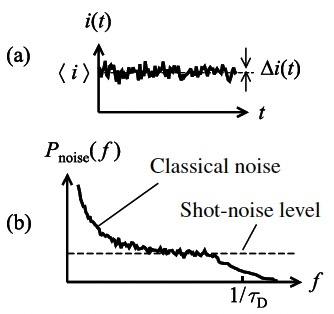
\includegraphics[width=0.35\textwidth]{figs/2022-05-08-09-51-35.png}
    \end{center}
    光源的经典噪声应来源于光源(激光器)的驱动电路及腔中镜片的热振动, 因此只出现在低率区. 高频区的噪声称为散粒噪声, 来源于光子统计. \\
    散粒噪声的特点: 
    \begin{enumerate}
        \item 电流方差与电流平均值成正比
        \item 噪声谱是白的,即不依赖于光子频率.
    \end{enumerate}
\end{frame}

\begin{frame} 
 \frametitle{* 增益与噪声}
      光电放大器的增益系数: $\gamma $ \\ 
      增益: G, 
      \[ G= \exp (\gamma L) \]
      (L 为光电信号线性区域的长度)\\
      信号-噪声率(SNR):
      \[\text{SNR}= \frac{\left\langle I \right\rangle^2}{\left (\langle \Delta I)^2 \right\rangle}  \]
\end{frame}

\begin{frame} 
 \frametitle{}
    量子化SNR: 
    \[\text{SNR}= \frac{\overline{n}}{\left (\langle \Delta n)^2 \right\rangle}  \]
    对于相干光:
    \[\text{SNR}= \frac{\overline{n}}{\left (\langle \Delta n)^2 \right\rangle} = \frac{\overline{n}}{\left (\langle \sqrt{\overline{n}})^2 \right\rangle} = \overline{n}\]  
    噪声系数 (NF): 
    \[\text{NF}=\frac{\text{SNR}_{in}}{\text{SNR}_{out}} = 2-\frac{1}{G} \]
\end{frame}

%%%%%%%%%%%%%%%%%%%%%%%%%%%%%%%%%%%%%%%%%%%%%%%%%%%%%%%%%%%%%%%%%%%
\begin{frame} 
    \frametitle{课外作业}
    A 10 mW He:Ne laser operating at 632.8 nm is detected with a photodiode of responsivity of 0.43 $AW^{−1}$ via a load resistor of 50 Ω. Calculate:
    \begin{enumerate}
        \item the quantum efficiency of the detector
        \item the average photocurrent
        \item the root-mean-square current fluctuations within a band-width of 100 kHz,
        \item  the noise power measured in dBm units after amplification by an
        amplifier with a power gain of 20 dB in the same 100 kHz bandwidth.
    \end{enumerate}
\end{frame}
%%%%%%%%%%%%%%%%%%%%%%%%%%%%%%%%%%%%%%%%%%%%%%%%%%%%%%%%%%%%%%%%%%%